\section{Exercises}


%_________________
\subsection{Case study}

% 1

\eoce{\qt{Migraine and acupuncture}
A migraine is a particularly painful type of headache, which patients sometimes wish to treat with acupuncture. To determine whether acupuncture relieves migraine pain, researchers conducted a randomized controlled study where 89 females diagnosed with migraine headaches were randomly assigned to one of two groups: treatment or control. 43 patients in the treatment group received acupuncture that is specifically designed to treat migraines. 46 patients in the control group received placebo acupuncture (needle insertion at nonacupoint locations). 24 hours after patients received acupuncture, they were asked if they were pain free. Results are summarized in the contingency table below. \footfullcite{Allais:2011}

\noindent\begin{minipage}[l]{0.4\textwidth}
\begin{tabular}{ll  cc c} 
			&				& \multicolumn{2}{c}{\textit{Pain free}} \\
\cline{3-4}
			&							& Yes 	& No 	& Total	\\
\cline{2-5}
							&Treatment 	& 10	 	& 33		& 43 	\\
\raisebox{1.5ex}[0pt]{\emph{Group}}	& Control		& 2	 	& 44 	 	& 46 \\
\cline{2-5}
							&Total		& 12		& 77		& 89
\end{tabular}
\end{minipage}
\begin{minipage}[c]{0.05\textwidth}
\end{minipage}
\begin{minipage}[c]{0.27\textwidth}
\begin{center}
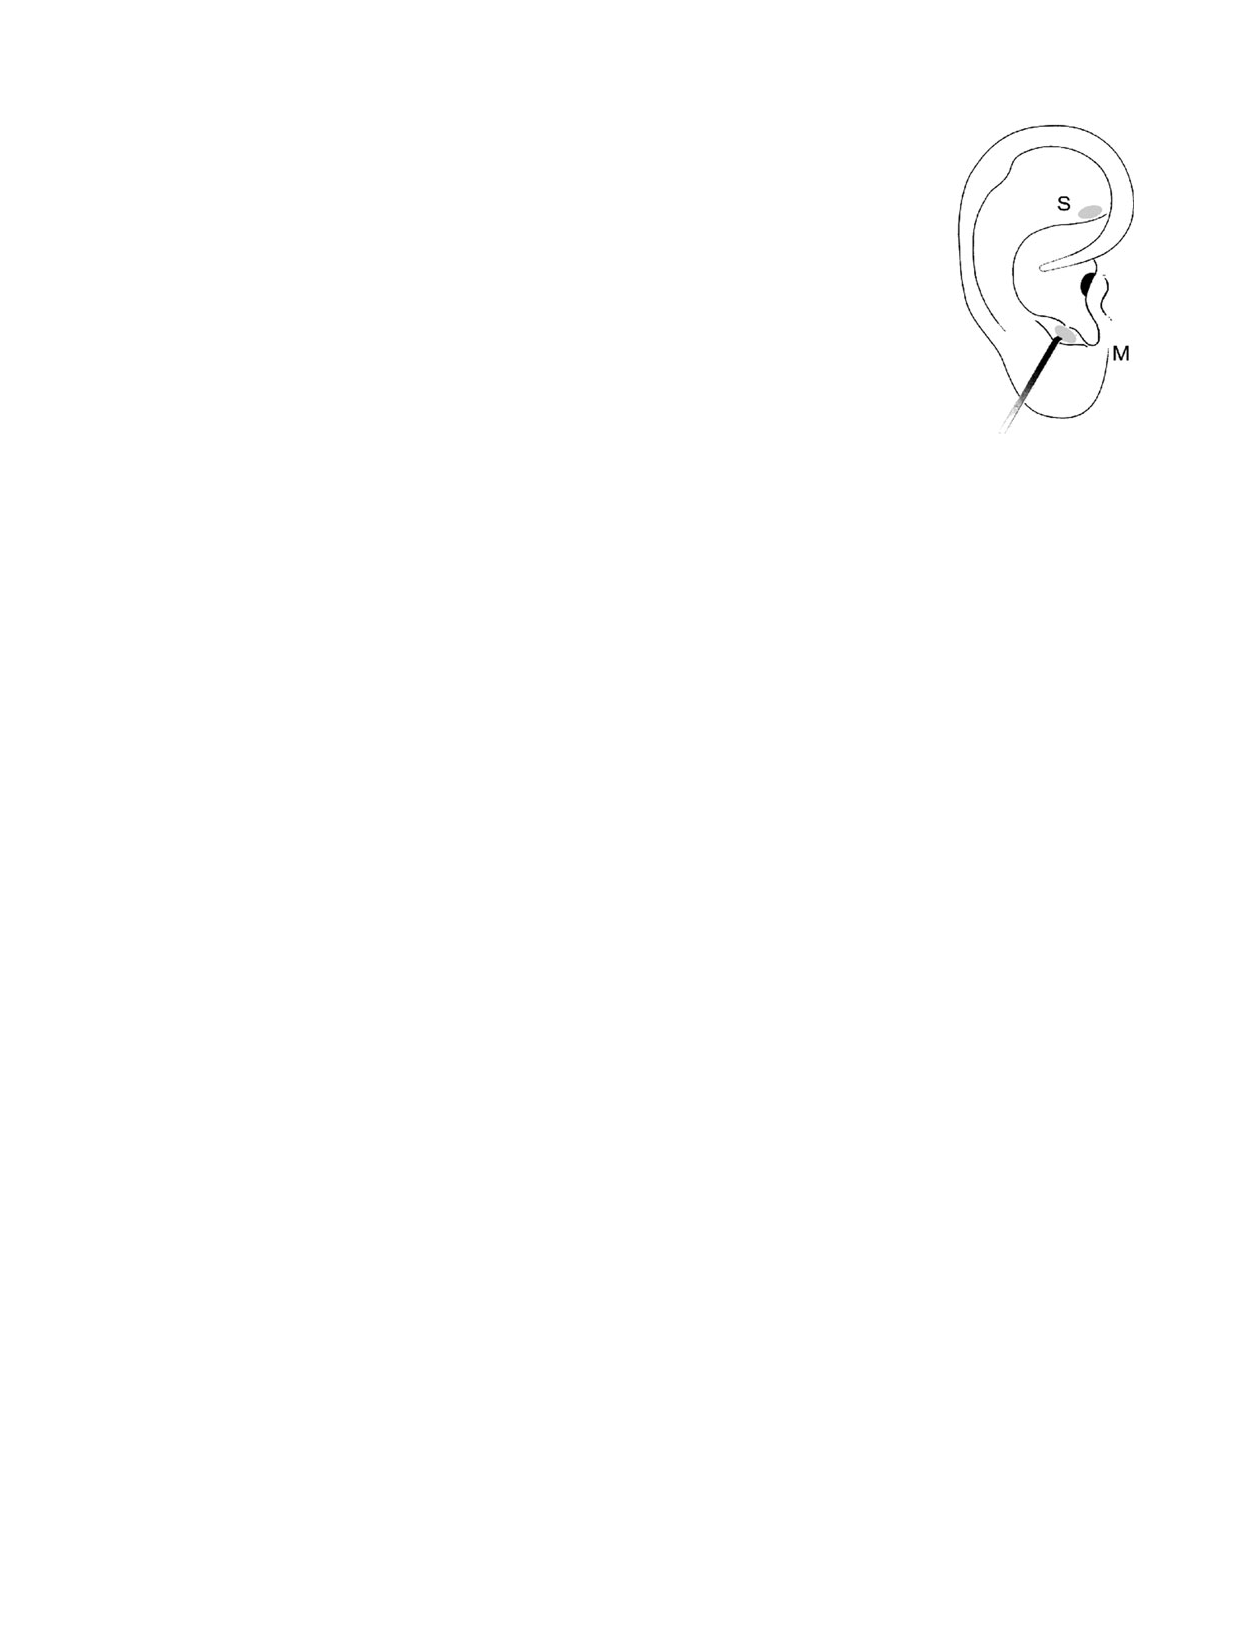
\includegraphics[width = 0.75\textwidth]{ch_data_collection/figures/eoce/images/earacupuncture}
\end{center}
\end{minipage}
\begin{minipage}[c]{0.25\textwidth}
{\footnotesize Figure from the original paper displaying the appropriate area (M) versus the inappropriate area (S) used in the treatment of migraine attacks.}
\end{minipage}
\begin{parts}
\item What percent of patients in the treatment group were pain free 24 hours after receiving acupuncture? What percent in the control group?
\item At first glance, does acupuncture appear to be an effective treatment for migraines? Explain your reasoning.
\item Do the data provide convincing evidence that there is a real pain reduction for those patients in the treatment group? Or do you think that the observed difference might just be due to chance?
\end{parts}
}
{}

% 2

\eoce{\qt{Sinusitis and antibiotics, Part I\label{sinusitis}} Researchers studying the effect of antibiotic treatment for acute sinusitis compared to symptomatic treatments randomly assigned 166 adults diagnosed with acute sinusitis to one of two groups: treatment or control. Study participants received either a 10-day course of amoxicillin (an antibiotic) or a placebo similar in appearance and taste. The placebo consisted of symptomatic treatments such as acetaminophen, nasal decongestants, etc. At the end of the 10-day period patients were asked if they experienced significant improvement in symptoms. The distribution of responses are summarized below. \footfullcite{Garbutt:2012}
\begin{center}
\begin{tabular}{ll  cc c} 
			&				& \multicolumn{2}{c}{\textit{Self-reported significant}} \\
			&				& \multicolumn{2}{c}{\textit{improvement in symptoms}} \\
\cline{3-4}
			&							& Yes 	& No 	& Total	\\
\cline{2-5}
							&Treatment 	& 66	 	& 19		& 85 	\\
\raisebox{1.5ex}[0pt]{\emph{Group}}	& Control		& 65	 	& 16 	 	& 81 \\
\cline{2-5}
							&Total		& 131	& 35		& 166
\end{tabular}
\end{center}
\begin{parts}
\item What percent of patients in the treatment group experienced a significant improvement in symptoms? What percent in the control group?
\item Based on your findings in part (a), which treatment appears to be more effective for sinusitis?
\item Do the data provide convincing evidence that there is a difference in the improvement rates of sinusitis symptoms? Or do you think that the observed difference might just be due to chance?
\end{parts}
}
{}


%_________________
\subsection{Data basics}

% 3

\eoce{\qt{Identify study components, Part I\label{components1}} Identify (i) the cases, (ii) the variables and their types, and (iii) the main research question in the studies described below.
\begin{parts}
\item Researchers collected data to examine the relationship between pollutants and preterm births in Southern California. During the study air pollution levels were measured by air quality monitoring stations. Specifically, levels of carbon monoxide were recorded in parts per million, nitrogen dioxide and ozone in parts per hundred million, and coarse particulate matter (PM$_{10}$) in $\mu g/m^3$. Length of gestation data were collected on 143,196 births between the years 1989 and 1993, and air pollution exposure during gestation was calculated for each birth. The analysis suggested that increased ambient PM$_{10}$ and, to a lesser degree, CO concentrations may be associated with the occurrence of preterm births. \footfullcite{Ritz+Yu+Chapa+Fruin:2000}
\item The Buteyko method is a shallow breathing technique developed by Konstantin Buteyko, a Russian doctor, in 1952. Anecdotal evidence suggests that the Buteyko method can reduce asthma symptoms and improve quality of life. In a scientific study to determine the effectiveness of this method, researchers recruited 600 asthma patients aged 18-69 who relied on medication for asthma treatment. These patients were split into two research groups: one practiced the Buteyko method and the other did not. Patients were scored on quality of life, activity, asthma symptoms, and medication reduction on a scale from 0 to 10. On average, the participants in the Buteyko group experienced a significant reduction in asthma symptoms and an improvement in quality of life. \footfullcite{McDowan:2003}
\end{parts}
}{}

% 4

\eoce{\qt{Identify study components, Part II\label{components2}} Identify (i) the cases, (ii) the variables and their types, and (iii) the main research question of the studies described below.
\begin{parts}
\item While obesity is measured based on body fat percentage (more than 35\% body fat for women and more than 25\% for men), precisely measuring body fat percentage is difficult. Body mass index (BMI), calculated as the ratio $weight/height^2$, is often used as an alternative indicator for obesity. A common criticism of BMI is that it assumes the same relative body fat percentage regardless of age, sex, or ethnicity. In order to determine how useful BMI is for predicting body fat percentage across age, sex and ethnic groups, researchers studied 202 black and 504 white adults who resided in or near New York City, were ages 20-94 years old, had BMIs of 18-35 kg/m$^2$, and who volunteered to be a part of the study. Participants reported their age, sex, and ethnicity and were measured for weight and height. Body fat percentage was measured by submerging the participants in water. \footfullcite{Gallagher:1996} \label{BMIAgeSexEth}

\item In a study of the relationship between socio-economic class and unethical behavior, 129 University of California undergraduates at Berkeley were asked to identify themselves as having low or high social-class by comparing themselves to others with the most (least) money, most (least) education, and most (least) respected jobs. They were also presented  with a jar of individually wrapped candies and informed that they were for children in a nearby laboratory, but that they could take some if they wanted. Participants completed unrelated tasks and then reported the number of candies they had taken. It was found that those in the upper-class rank condition took more candy than did those in the lower-rank condition. \footfullcite{Piff:2012}
\end{parts}
}{}

% 5
\textPE{\pagebreak}

\eoce{\qt{Fisher's irises} Sir Ronald Aylmer Fisher was an English statistician, evolutionary biologist, and geneticist who worked on a data set that contained sepal length and width, and petal length and width from three species of iris flowers (\textit{setosa}, \textit{versicolor} and \textit{virginica}). There were 50 flowers from each species in the data set. \footfullcite{Fisher:1936,irisPic} \\
\noindent\begin{minipage}[c]{0.55\textwidth}
\begin{parts}
\item How many cases were included in the data?
\item How many numerical variables are included in the data? Indicate what they are, and if they are continuous or discrete.
\item How many categorical variables are included in the data, and what are they? List the corresponding levels (categories).
\end{parts} \vspaceB{10mm}
\end{minipage}
\begin{minipage}[c]{0.4\textwidth}
\begin{center}
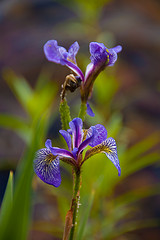
\includegraphics[width = 30mm]{ch_data_collection/figures/eoce/images/irisversicolor}
\end{center}
\end{minipage}
}{}

% 6

\eoce{\qt{Smoking habits of UK residents\label{UKSmoking_datamatrix}} A survey was conducted to study the smoking habits of UK residents. Below is a data matrix displaying a portion of the data collected in this survey. Note that ``$\pounds$" stands for British Pounds Sterling, ``cig" stands for cigarettes, and ``N/A'' refers to a missing component of the data. \footfullcite{data:smoking}
\begin{table}[h]
\begin{center}
\scriptsize{
\begin{tabular}{rccccccc}
  \hline
 & gender & age & marital & grossIncome & smoke & amtWeekends & amtWeekdays \\ 
  \hline
1 & Female &  42 & Single & Under $\pounds$2,600 & Yes &  12 cig/day &  12 cig/day \\ 
2 & Male &  44 & Single & $\pounds$10,400 to $\pounds$15,600 & No & N/A & N/A \\ 
3 & Male &  53 & Married & Above $\pounds$36,400 & Yes &   6 cig/day &   6 cig/day \\ 
\vdots & \vdots &  \vdots & \vdots & \vdots & \vdots & \vdots & \vdots \\ 
1691 & Male &  40 & Single & $\pounds$2,600 to $\pounds$5,200 & Yes &   8 cig/day &   8 cig/day \\   
   \hline
\end{tabular}
}
\end{center}
\end{table}
\begin{parts}
\item What does each row of the data matrix represent?
\item How many participants were included in the survey?
\item Indicate whether each variable in the study is numerical or categorical. If numerical, identify as continuous or discrete. If categorical, indicate if the variable is ordinal.
\end{parts}
}{}


%_________________
\subsection{Overview of data collection principles}

% 7

\eoce{\qt{Generalizability and causality, Part I} Identify the population of interest and the sample in the studies described in Exercise~\ref{components1}. Comment on whether or not the results of the study can be generalized to the population and if the findings of the study can be used to establish causal relationships.
}{}

% 8

\eoce{\qt{Generalizability and causality, Part II} Identify the population of interest and the sample in the studies described in Exercise~\ref{components2}. Comment on whether or not the results of the study can be generalized to the population and if the findings of the study can be used to establish causal relationships.
}{}

% 9
\textPE{\pagebreak}

\eoce{\qt{GPA and study time} A survey was conducted on 218 undergraduates from Duke University who took an introductory statistics course in Spring 2012. Among many other questions, this survey asked them about their GPA and the number of hours they spent studying per week. The scatterplot below displays the relationship between these two variables.

\noindent\begin{minipage}[c]{0.44\textwidth}
\begin{parts}
\item What is the explanatory variable and what is the response variable?
\item Describe the relationship between the two variables. Make sure to discuss unusual observations, if any.
\item Is this an experiment or an observational study?
\item Can we conclude that studying longer hours leads to higher GPAs?
\end{parts} \vspaceB{4mm}
\end{minipage}
\begin{minipage}[c]{0.55\textwidth}
\begin{center}
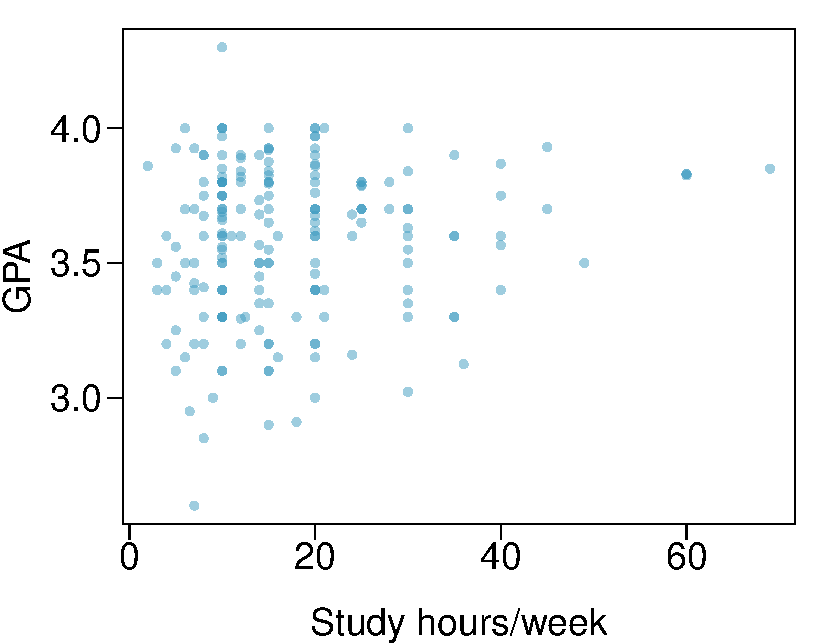
\includegraphics[width = 0.88\textwidth]{ch_data_collection/figures/eoce/gpaStudy/gpaStudy}
\end{center}
\end{minipage}
}{}


% 10

\eoce{\qt{Income and education} The scatterplot below shows the relationship between per capita income (in thousands of dollars) and percent of population with a bachelor's degree in 3,143 counties in the US in 2010.

\noindent\begin{minipage}[c]{0.44\textwidth}
\begin{parts}
\item What are the explanatory and response variables?
\item Describe the relationship between the two variables. Make sure to discuss unusual observations, if any.
\item Can we conclude that having a bachelor's degree increases one's income?
\end{parts} \vspaceB{16mm}
\end{minipage}
\begin{minipage}[c]{0.55\textwidth}
\begin{center}
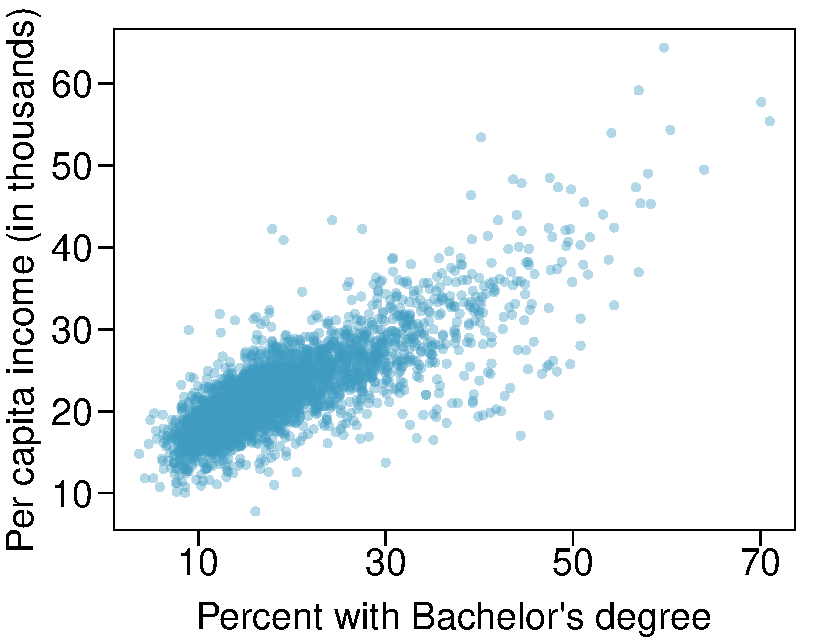
\includegraphics[width = 0.88\textwidth]{ch_data_collection/figures/eoce/county/county_incomeBach}
\end{center}
\end{minipage}
}{}


%_________________
\subsection{Observational studies and sampling strategies}

% 11

\eoce{\qt{Propose a sampling strategy} A large college class has 160 students. All 160 students attend the lectures together, but the students are divided into 4 groups, each of 40 students, for lab sections administered by different teaching assistants. The professor wants to conduct a survey about how satisfied the students are with the course, and he believes that the lab section a student is in might affect the student's overall satisfaction with the course.
\begin{parts}
\item What type of study is this?
\item Suggest a sampling strategy for carrying out this study.
\end{parts}
}{}


% 12
\textPE{\pagebreak}

\eoce{\qt{Internet use and life expectancy} The scatterplot below shows the relationship between estimated life expectancy at birth as of 2012\footfullcite{data:ciaFactBookLifeExp:2012} and percentage of internet users in 2010\footfullcite{data:ITU:2012} in 208 countries.

\noindent\begin{minipage}[c]{0.43\textwidth}
\begin{parts}
\item Describe the relationship between life expectancy and percentage of internet users.
\item What type of study is this?
\item State a possible confounding variable that might explain this relationship and describe its potential effect.
\end{parts}\vspace{16mm}
\end{minipage}%
\begin{minipage}[r]{0.55\textwidth}
\hfill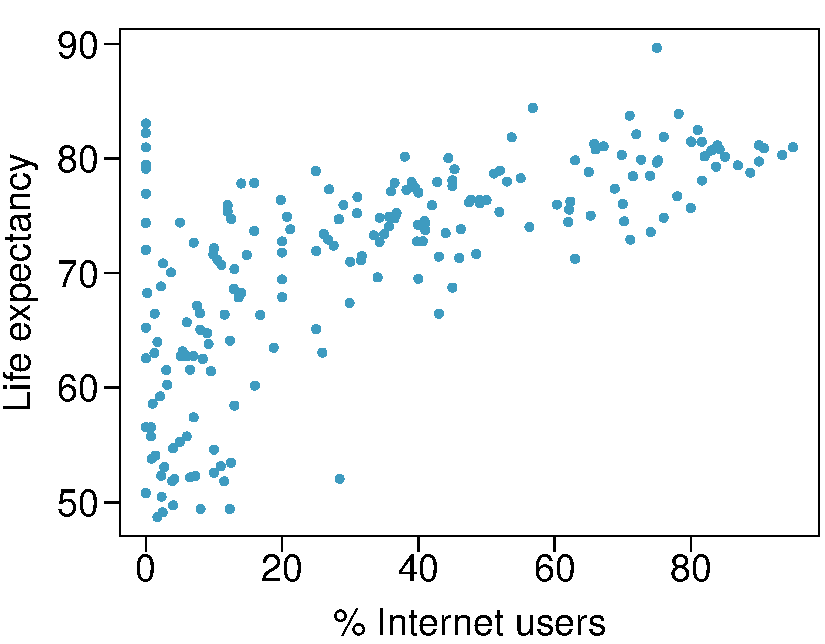
\includegraphics[width = 0.95\textwidth]{ch_data_collection/figures/eoce/country/county_lifeExpInter}
\end{minipage}
}{}

% 13

\eoce{\qt{Random digit dialing} The Gallup Poll uses a procedure called random digit dialing, which creates phone numbers based on a list of all area codes in America in conjunction with the associated number of residential households in each area code. Give a possible reason the Gallup Poll chooses to use random digit dialing instead of picking phone numbers from the phone book.
}{}

% 14

\eoce{\qt{Sampling strategies} A statistics student who is curious about the relationship between the amount of time students spend on social networking sites and their performance at school decides to conduct a survey. Three research strategies for collecting data are described below. In each, name the sampling method proposed and any bias you might expect.
\begin{parts}
\item He randomly samples 40 students from the study's population, gives them the survey, asks them to fill it out and bring it back the next day.
\item He gives out the survey only to his friends, and makes sure each one of them fills out the survey.
\item He posts a link to an online survey on his Facebook wall and asks his friends to fill out the survey.
\APVersion{\item He stands outside the student center and asks every third person that walks out the door to fill out the survey.}
\end{parts}
}{}


% 15

\eoce{\qt{Family size} Suppose we want to estimate family size, where family is defined as one or more parents living with children. If we select students at random at an elementary school and ask them what their family size is, will our average be biased? If so, will it overestimate or underestimate the true value?
}{}


\textPE{\newpage}

% 16

\eoce{\qt{Flawed reasoning} Identify the flaw in reasoning in the following scenarios. Explain what the individuals in the study should have done differently if they wanted to make such strong conclusions.
\begin{parts}
\item Students at an elementary school are given a questionnaire that they are required to return after their parents have completed it. One of the questions asked is, ``Do you find that your work schedule makes it difficult for you to spend time with your kids after school?" Of the parents who replied, 85\% said ``no". Based on these results, the school officials conclude that a great majority of the parents have no difficulty spending time with their kids after school.
\item A survey is conducted on a simple random sample of 1,000 women who recently gave birth, asking them about whether or not they smoked during pregnancy. A follow-up survey asking if the children have respiratory problems is conducted 3 years later, however, only 567 of these women are reached at the same address. The researcher reports that these 567 women are representative of all mothers.
\item A orthopedist administers a questionnaire to 30 of his patients who do not have any joint problems and finds that 20 of them regularly go running. He concludes that running decreases the risk of joint problems.
\end{parts}
}{}


% 17

\eoce{\qt{Reading the paper} Below are excerpts from two articles published in the \emph{NY Times}:
\begin{parts}
\item An article called \emph{Risks: Smokers Found More Prone to Dementia} states the following: \footfullcite{news:smokingDementia}
\begin{adjustwidth}{2em}{2em}
{\footnotesize ``Researchers analyzed the data of 23,123 health plan members who participated in a voluntary exam and health behavior survey from 1978 to 1985, when they were 50 to 60 years old. Twenty-three years later, about one-quarter of the group, or 5,367, had dementia, including 1,136 with Alzheimer�s disease and 416 with vascular dementia. After adjusting for other factors, the researchers concluded that pack-a-day smokers were 37 percent more likely than nonsmokers to develop dementia, and the risks went up sharply with increased smoking; 44 percent for one to two packs a day; and twice the risk for more than two packs."}
\end{adjustwidth}
Based on this study, can we conclude that smoking causes dementia later in life? Explain your reasoning.
\item Another article called \emph{The School Bully Is Sleepy} states the following: \footfullcite{news:bullySleep}
\begin{adjustwidth}{2em}{2em}
{\footnotesize ``The University of Michigan study, collected survey data from parents on each child's sleep habits and asked both parents and teachers to assess behavioral concerns. About a third of the students studied were identified by parents or teachers as having problems with disruptive behavior or bullying. The researchers found that children who had behavioral issues and those who were identified as bullies were twice as likely to have shown symptoms of sleep disorders."}
\end{adjustwidth}
A friend of yours who read the article says, ``The study shows that sleep disorders lead to bullying in school children." Is this statement justified? If not, how best can you describe the conclusion that can be drawn from this study?
\end{parts}
}{}


% 18

\eoce{\qt{Shyness on Facebook} Given the anonymity afforded to individuals in online interactions, researchers hypothesized that shy individuals would have more favorable attitudes toward Facebook and that shyness would be positively correlated with time spent on Facebook. They also hypothesized that shy individuals would have fewer Facebook ``Friends" just like they have fewer friends than non-shy individuals have in the offline world. Data were collected on 103 undergraduate students at a university in southwestern Ontario via online questionnaires. The study states ``Participants were recruited through the university's psychology participation pool. After indicating an interest in the
study, participants were sent an e-mail containing the study's URL as well as the necessary login credentials." Are the results of this study generalizable to the population of all Facebook users? \footfullcite{Orr:2009}
}{}


%_________________
\textPE{\pagebreak}
\subsection{Experiments}

% 19

\eoce{\qt{Vitamin supplements} In order to assess the effectiveness of taking large doses of vitamin C in reducing the duration of the common cold, researchers recruited 400 healthy volunteers from staff and students at a university. A quarter of the patients were assigned a placebo, and the rest were evenly divided between 1g Vitamin C,  3g Vitamin C, or 3g Vitamin C plus additives to be taken at onset of a cold for the following two days. All tablets had identical appearance and packaging. The nurses who handed the prescribed pills to the patients knew which patient received which treatment, but the researchers assessing the patients when they were sick did not. No significant differences were observed in any measure of cold duration or severity between the four medication groups, and the placebo group had the shortest duration of symptoms.\footfullcite{Audera:2001}
\begin{parts}
\item Was this an experiment or an observational study? Why?
\item What are the explanatory and response variables in this study?
\item Were the patients blinded to their treatment?
\item Was this study double-blind?
\item Participants are ultimately able to choose whether or not to use the pills prescribed to them. We might expect that not all of them will adhere and take their pills. Does this introduce a confounding variable to the study? Explain your reasoning.
\end{parts}
}{}


% 20

\eoce{\qt{Soda preference} You would like to conduct an experiment in class to see if your classmates prefer the taste of regular Coke or Diet Coke. Briefly outline a design for this study.
}{}


% 21

\eoce{\qt{Exercise and mental health} A researcher is interested in the effects of exercise on mental health and he proposes the following study: Use stratified random sampling to ensure representative proportions of 18-30, 31-40 and 41-55 year olds from the population. Next, randomly assign half the subjects from each age group to exercise twice a week, and instruct the rest not to exercise. Conduct a mental health exam at the beginning and at the end of the study, and compare the results.
\begin{parts}
\item What type of study is this? 
\item What are the treatment and control groups in this study?
\item Does this study make use of blocking? If so, what is the blocking variable?
\item Does this study make use of blinding?
\item Comment on whether or not the results of the study can be used to establish a causal relationship between exercise and mental health, and indicate whether or not the conclusions can be generalized to the population at large.
\item Suppose you are given the task of determining if this proposed study should get funding. Would you have any reservations about the study proposal?
\end{parts}
}{}


% 22
\textPE{\newpage}

\eoce{\qt{Chia seeds and weight loss} Chia Pets -- those terra-cotta figurines that sprout fuzzy green hair -- made the chia plant a household name. But chia has gained an entirely new reputation as a diet supplement.  In one 2009 study, a team of researchers recruited 38 men and divided them evenly into two groups: treatment or control. They also recruited 38 women, and they randomly placed half of these participants into the treatment group and the other half into the control group. One group was given 25 grams of chia seeds twice a day, and the other was given a placebo. The subjects volunteered to be a part of the study. After 12 weeks, the scientists found no significant difference between the groups in appetite or weight loss. \footfullcite{Nieman:2009}
\begin{parts}
\item What type of study is this? 
\item What are the experimental and control treatments in this study?
\item Has blocking been used in this study? If so, what is the blocking variable?
\item Has blinding been used in this study?
\item Comment on whether or not we can make a causal statement, and indicate whether or not we can generalize the conclusion to the population at large.
\end{parts}
}{}
